%  LaTeX support: latex@mdpi.com
%  In case you need support, please attach all files that are necessary for compiling as well as the log file, and specify the details of your LaTeX setup (which operating system and LaTeX version / tools you are using).

%=================================================================
\documentclass[agronomy,article,submit,moreauthors,pdftex]{mdpi}

% If you would like to post an early version of this manuscript as a preprint, you may use preprint as the journal and change 'submit' to 'accept'. The document class line would be, e.g., \documentclass[preprints,article,accept,moreauthors,pdftex]{mdpi}. This is especially recommended for submission to arXiv, where line numbers should be removed before posting. For preprints.org, the editorial staff will make this change immediately prior to posting.

%% Some pieces required from the pandoc template
\providecommand{\tightlist}{%
  \setlength{\itemsep}{0pt}\setlength{\parskip}{4pt}}
\setlist[itemize]{leftmargin=*,labelsep=5.8mm}
\setlist[enumerate]{leftmargin=*,labelsep=4.9mm}

\usepackage{longtable}

% see https://stackoverflow.com/a/47122900

%--------------------
% Class Options:
%--------------------
%----------
% journal
%----------
% Choose between the following MDPI journals:
% acoustics, actuators, addictions, admsci, aerospace, agriculture, agriengineering, agronomy, ai, algorithms, allergies, analytica, animals, antibiotics, antibodies, antioxidants, applmech, applnano, applsci, arts, asc, asi, atmosphere, atoms, automation, axioms, batteries, bdcc, behavsci , beverages, bioengineering, biology, biomedicines, biomedinformatics, biomimetics, biomolecules, biosensors, bloods, brainsci, breath, buildings, cancers, carbon , catalysts, cells, ceramics, challenges, chemengineering, chemistry, chemosensors, chemproc, children, civileng, cleantechnol, climate, clockssleep, cmd, coatings, colloids, computation, computers, condensedmatter, cosmetics, cryptography, crystals, cyber, dairy, data, dentistry, dermatopathology, designs, diabetology, diagnostics, digital, diseases, diversity, drones, earth, econometrics, ecologies, economies, education, ejbc, ejihpe, electricity, electrochem, electronicmat, electronics, endocrines, energies, engproc, entropy, environments, environsciproc, epidemiologia, epigenomes, est, fermentation, fibers, fire, fishes, fluids, foods, forecasting, forests, fractalfract, fuels, futureinternet, futurephys, galaxies, games, gardens, gases, gastrointestdisord, gels, genealogy, genes, geohazards, geosciences, geriatrics, hazardousmatters, healthcare, hearts, heritage, highthroughput, horticulturae, humanities, hydrogen, hydrology, ijerph, ijfs, ijgi, ijms, ijtpp, immuno, informatics, information, infrastructures, inorganics, insects, instruments, inventions, iot, j, jcdd, jce, jcm, jcp, jcs, jdb, jfb, jfmk, jimaging, jintelligence, jlpea, jmmp, jmse, jne, jnt, jof, joitmc, journalmedia, jpm, jrfm, jsan, land, languages, laws, life, literature, livers, logistics, lubricants, machines, magnetochemistry, make, marinedrugs, materials, materproc, mathematics, mca, medicina, medicines, medsci, membranes, metabolites, metals, microarrays, micromachines, microorganisms, minerals, modelling, molbank, molecules, mps, mti, nanomaterials, ncrna, ijns, neurosci, neuroglia, nitrogen, notspecified, nutrients, obesities, oceans, ohbm, osteology, optics, organics, particles, pathogens, pharmaceuticals, pharmaceutics, pharmacy, philosophies, photonics, physics, plants, plasma, pollutants, polymers, polysaccharides, preprints , proceedings, processes, prosthesis, proteomes, psych, psychiatryint, publications, quantumrep, quaternary, qubs, radiation, reactions, recycling, religions, remotesensing, reprodmed, reports, resources, risks, robotics, safety, sci, scipharm, sensors, separations, sexes, signals, sinusitis, skins, smartcities, sna, societies, socsci, soilsystems, solids, sports, standards, stats, surfaces, surgeries, suschem, sustainability, world, symmetry, systems, technologies, telecom, test, tourismhosp, toxics, toxins, transplantology, tropicalmed, universe, urbansci, uro, vaccines, vehicles, vetsci, vibration, viruses, vision, water, wem, wevj, women

%---------
% article
%---------
% The default type of manuscript is "article", but can be replaced by:
% abstract, addendum, article, benchmark, book, bookreview, briefreport, casereport, changes, comment, commentary, communication, conceptpaper, conferenceproceedings, correction, conferencereport, expressionofconcern, extendedabstract, meetingreport, creative, datadescriptor, discussion, editorial, essay, erratum, hypothesis, interestingimages, letter, meetingreport, newbookreceived, obituary, opinion, projectreport, reply, retraction, review, perspective, protocol, shortnote, supfile, technicalnote, viewpoint
% supfile = supplementary materials

%----------
% submit
%----------
% The class option "submit" will be changed to "accept" by the Editorial Office when the paper is accepted. This will only make changes to the frontpage (e.g., the logo of the journal will get visible), the headings, and the copyright information. Also, line numbering will be removed. Journal info and pagination for accepted papers will also be assigned by the Editorial Office.

%------------------
% moreauthors
%------------------
% If there is only one author the class option oneauthor should be used. Otherwise use the class option moreauthors.

%---------
% pdftex
%---------
% The option pdftex is for use with pdfLaTeX. If eps figures are used, remove the option pdftex and use LaTeX and dvi2pdf.

%=================================================================
\firstpage{1}
\makeatletter
\setcounter{page}{\@firstpage}
\makeatother
\pubvolume{xx}
\issuenum{1}
\articlenumber{5}
\pubyear{2020}
\copyrightyear{2020}
%\externaleditor{Academic Editor: name}
\history{Received: date; Accepted: date; Published: date}
\updates{yes} % If there is an update available, un-comment this line

%% MDPI internal command: uncomment if new journal that already uses continuous page numbers
%\continuouspages{yes}

%------------------------------------------------------------------
% The following line should be uncommented if the LaTeX file is uploaded to arXiv.org
%\pdfoutput=1

%=================================================================
% Add packages and commands here. The following packages are loaded in our class file: fontenc, calc, indentfirst, fancyhdr, graphicx, lastpage, ifthen, lineno, float, amsmath, setspace, enumitem, mathpazo, booktabs, titlesec, etoolbox, amsthm, hyphenat, natbib, hyperref, footmisc, geometry, caption, url, mdframed, tabto, soul, multirow, microtype, tikz

%=================================================================
%% Please use the following mathematics environments: Theorem, Lemma, Corollary, Proposition, Characterization, Property, Problem, Example, ExamplesandDefinitions, Hypothesis, Remark, Definition
%% For proofs, please use the proof environment (the amsthm package is loaded by the MDPI class).

%=================================================================
% Full title of the paper (Capitalized)
\Title{A meta-analysis of fungicide spray schedules to minimise yield
loss from powdery mildew in Australian mungbean}

% Authors, for the paper (add full first names)
\Author{Paul
Melloy$^{1,*}$\href{https://orcid.org/0000-0003-4253-7167}{\orcidicon}, Emerson
Del
Ponte$^{2}$\href{https://orcid.org/0000-0003-4398-409X}{\orcidicon}, Adam
H. Sparks$^{3}$\href{https://orcid.org/0000-0002-0061-8359}{\orcidicon}}

% Authors, for metadata in PDF
\AuthorNames{Paul Melloy, Emerson Del Ponte, Adam H. Sparks}

% Affiliations / Addresses (Add [1] after \address if there is only one affiliation.)
\address{%
$^{1}$ \quad University of Southern Queensland Centre for Crop Health
Toowoomba, Queensland, 4350
Australia; \href{mailto:Paul.Melloy@usq.edu.au}{\nolinkurl{Paul.Melloy@usq.edu.au}}\\
$^{2}$ \quad Universidade Federal de Viçosa Departamento de
Fitopatologia Viçosa, 36570-000 Minas Gearais,
Brazil; \href{mailto:delponte@ufv.br}{\nolinkurl{delponte@ufv.br}}\\
$^{3}$ \quad University of Southern Queensland Centre for Crop Health
Toowoomba, Queensland, 4350
Australia; \href{mailto:Adam.Sparks@usq.edu.au}{\nolinkurl{Adam.Sparks@usq.edu.au}}\\
}
% Contact information of the corresponding author
\corres{Correspondence: \href{mailto:Paul.Melloy@usq.edu.au}{\nolinkurl{Paul.Melloy@usq.edu.au}};
Tel.: +61 7 4631 5527}

% Current address and/or shared authorship








% The commands \thirdnote{} till \eighthnote{} are available for further notes

% Simple summary
\simplesumm{A simple summary goes here.}

% Abstract (Do not insert blank lines, i.e. \\)
\abstract{A single paragraph of about 200 words maximum. For research
articles, abstracts should give a pertinent overview of the work. We
strongly encourage authors to use the following style of structured
abstracts, but without headings: 1) Background: Place the question
addressed in a broad context and highlight the purpose of the study; 2)
Methods: Describe briefly the main methods or treatments applied; 3)
Results: Summarize the article's main findings; and 4) Conclusion:
Indicate the main conclusions or interpretations. The abstract should be
an objective representation of the article, it must not contain results
which are not presented and substantiated in the main text and should
not exaggerate the main conclusions.}

% Keywords
\keyword{keyword 1; keyword 2; keyword 3 (list three to ten pertinent
keywords specific to the article, yet reasonably common within the
subject discipline.).}

% The fields PACS, MSC, and JEL may be left empty or commented out if not applicable
%\PACS{J0101}
%\MSC{}
%\JEL{}

%%%%%%%%%%%%%%%%%%%%%%%%%%%%%%%%%%%%%%%%%%
% Only for the journal Diversity
%\LSID{\url{http://}}

%%%%%%%%%%%%%%%%%%%%%%%%%%%%%%%%%%%%%%%%%%
% Only for the journal Applied Sciences:
%\featuredapplication{Authors are encouraged to provide a concise description of the specific application or a potential application of the work. This section is not mandatory.}
%%%%%%%%%%%%%%%%%%%%%%%%%%%%%%%%%%%%%%%%%%

%%%%%%%%%%%%%%%%%%%%%%%%%%%%%%%%%%%%%%%%%%
% Only for the journal Data:
%\dataset{DOI number or link to the deposited data set in cases where the data set is published or set to be published separately. If the data set is submitted and will be published as a supplement to this paper in the journal Data, this field will be filled by the editors of the journal. In this case, please make sure to submit the data set as a supplement when entering your manuscript into our manuscript editorial system.}

%\datasetlicense{license under which the data set is made available (CC0, CC-BY, CC-BY-SA, CC-BY-NC, etc.)}

%%%%%%%%%%%%%%%%%%%%%%%%%%%%%%%%%%%%%%%%%%
% Only for the journal Toxins
%\keycontribution{The breakthroughs or highlights of the manuscript. Authors can write one or two sentences to describe the most important part of the paper.}

%\setcounter{secnumdepth}{4}
%%%%%%%%%%%%%%%%%%%%%%%%%%%%%%%%%%%%%%%%%%


\usepackage{booktabs}
\usepackage{longtable}
\usepackage{array}
\usepackage{multirow}
\usepackage{wrapfig}
\usepackage{float}
\usepackage{colortbl}
\usepackage{pdflscape}
\usepackage{tabu}
\usepackage{threeparttable}
\usepackage{threeparttablex}
\usepackage[normalem]{ulem}
\usepackage{makecell}
\usepackage{xcolor}

\begin{document}
%%%%%%%%%%%%%%%%%%%%%%%%%%%%%%%%%%%%%%%%%%

Mungbean {[}\emph{Vigna radiata} (L.) Wilczek{]} is a pulse crop
primarily grown in south-east Asia for human consumption as an
affordable source of protein \citep{Lambrides2007}. The bean pod or
grain can be consumed raw or added to meals after sprouting. The dried
grain can also be ground into a protein enriched flour for uses in
noodles, biscuits and cakes \citep{Chankaew2013}.

Mungbean was first brought to Australia in the 1930s for use as a forage
or green manure crop. However, it was only somewhat recently, the 1960s
that mungbean was grown commercially \citep{Lawn1978, Chauhan2018}.
Prior to the 1970s the total area grown in Australia rarely exceeded
1000 hectares \citep{Lawn1978}. At the end of the 1980s, between 3,000
to 10,0000 hectares were being harvested for dried beans in Australia,
of which mungbean is categorised by the FAO statistics data repository
\citep{FAOSTAT}. In the decade leading up to 2018 between 35 - 86.4
thousand hectares of dried beans were planted annually. This increase is
attributed high value export markets and to the improved yields in the
new cultivars \citep{Clarry2016}. Currently mungbean is predominantly
grown in southern Queensland and northern New South Wales as a short
season summer legume crop. In 2019, approximately 90~\% of Australian
mungbean was grown for export with lucrative returns of up to \$1300~AU
a tonne \citep{QueenslandGovernment2019}. Mungbean potentially yields up
to 3 tonnes per hectare \citep{ThomasRobert2004}, but due to high
variability in yields between seasons and locations, the average
Australian farm still yields less than 1 tonne per hectare
\citep{Chauhan2018}.

The high variability in yields, in part, can be attributed to a range of
diseases that affect the crop \citep{Kelly2017a}. Two major foliar
diseases, tan spot or common wilt (\emph{Curtobacterium flaccumfaciens}
pv. \emph{flaccumfaciens}) and halo blight (\emph{Pseudomonas
savastanoi} pv. \emph{phaseolicola}), are the main focus of the
Australian Mungbean Improvement programme's resistance breeding efforts
due to lack of effective chemical controls for them. While a third
disease, powdery mildew, can reduce yields by up to 40\%
\citep{Chankaew2013} in susceptible cultivars, the damage can be
mitigated through an integrated disease management strategy of fungicide
treatments and cultural practices.

Powdery mildew is caused by two separate genera of fungi in Australia
\emph{Podosphaera xanthii} and an unnamed \emph{Psuedoidium sp.} (Kiss
and Kelly Personal Communication). While the pathogens are obligate
parasites, secondary hosts that allow the pathogens to over-season
between mungbean crops have not yet been identified. The disease
lifecycle can be as short as five days for a germinating conidia to
infect the host and produce new reproductive structures, conidiophores,
which produce more conidia, which disseminate to new infection sites
\citep{Sparks2017}. Weather conditions that favour the rapid development
of the disease are cool temperatures between 22° and 26°C, and a leaf
surface that is not overly wet for infection \citep{Kelly2017a}.

Due to the requirement for cooler temperatures for infection, planting
date is an effective strategy for preventing the development of powdery
mildew in mungbean \citep{AMAplanting}. In southern Queensland and
northern New South Wales, sowing dates between late spring (November)
and mid-summer (January) are advised to avoid the conducive cooler
autumn temperatures, which normally commence in March. Therefore, a
delayed sowing date of late January into February increases the
possibility powdery mildew will infect earlier in the crop development
cycle and cause greater yield losses than in earlier sown mungbean
crops.

Cultivar selection is an additional strategy to mitigate yield damage
from powdery mildew. In Australia, quantitative resistance to powdery
mildew has also been incorporated into few commercially available
varieties. Jade-AU {(pbr)} has the the best disease resistance to
powdery mildew (moderately susceptible), with cv. Green Diamond also
containing some notable resistance \citep{Sparks2017}. However
commercially available mungbean cultivars in Australia lack sufficient
resistance to be used as the primary powdery mildew management strategy.
Evidence of this is shown by the 2016 field trials with the moderately
susceptible cultivar, Jade-AU, where yield losses of up to 32.7 \% were
recorded \citep{SueThompson2016}. Quantitative disease resistance has
been observed in some breeding lines overseas
\citep{Pandey2018, Chankaew2013}, however no evidence for how they
compare to Australian varietal resistance could be found. Additional
strategies to cultivar choice, such as fungicide treatments, are
necessary to limit yield loss when conditions for the disease are
conducive.

There is almost a complete lack of peer-reviewed literature summarising
fungicide efficacy on powdery mildew in Australian mungbean. Much of the
experimental work has been published by funding agencies and state
government extension departments as extension bulletins or other related
type materials. Past field trials in eastern Australia have tested a
range of fungicide active ingredients while also attempting to evaluate
the best application time for the highest efficacy
\citep{goolhi2013, premer2013, Millmerran2013, Marysmount2013, SueThompson2016, Kelly2017a, Thompson2016}.
Early trials showed that for fungicide applications to protect yield, a
single fungicide application at first sign of the disease with another
follow-up application two weeks later, if necessary, was the most
effective \citep{SueThompson2016, Sparks2017}. However, due to the
variability in the results between seasons and experiments, few of these
studies produced a clear result based on a statistical analysis. This
variability presents uncertainty for the best practice of fungicide
spray schedules to mitigate yield losses from powdery mildew.

The collection of experiments mentioned above and other unpublished
trials present an excellent opportunity for a meta-analysis.
Meta-analyses are statistical tools, which can analyse a collection of
experiments, that have a similar aim, and produces a more accurate
estimate of the true effect being measured. Using a meta-analysis can be
useful in situations like this where several studies exist, that have
the same objective but may not provide a clear answer to the question
due to variation in the results within the individual studies. The
outcome of a meta-analysis provides a more accurate estimation of the
true treatments effect, because it considers the amount of variance in
each study and weights the influence of each studies treatment effects
according to it's statistical accuracy. Typically meta-analyses consider
the effect of a single treatment against a control group across multiple
independent studies \citep{Madden2011}. However meta-analyses can also
consider effect differences between multiple treatments and a control
group, these are called multi-variate or network meta-analyses
\citep{MaddenEtAl2016}. Multi-variate meta-analyses are particularly
useful when there are no direct comparisons between two treatments in
any of the included studies. Indirect comparisons can be made between
these two treatments if the both had direct comparisons with one or more
treatments in common, assuming no significant bias in the studies that
investigated each of the treatments and which are subject to a indirect
comparison \citep{Jansen2011}.

Considering the recent launch in 2019 of the decision support system
(DSS) PowderyMildewMBM \citep{Diggle}, which provides a cost benefit
analysis to assists growers in their decision `if' and `when' apply
fungicide; a meta-analysis to evaluate and verify the best fungicide
spray schedule seemed prudent. The aim of this meta-analysis was to
determine, from a collection of unpublished studies, what spray
management scenario provides the greatest yield protection from powdery
mildew in Australian mungbean.

\hypertarget{materials-and-methods}{%
\section{Materials and Methods}\label{materials-and-methods}}

\hypertarget{trial-criteria-for-inclusion-and-description}{%
\subsection{Trial criteria for inclusion and
description}\label{trial-criteria-for-inclusion-and-description}}

The data for this study were obtained through personal correspondence
with colleagues and collaborating institutions. Trials undertaken in the
2013 season were conducted by the Northern Growers Alliance (NGA)
\citetext{\citeyear{goolhi2013}; \citeyear{premer2013}; \citeyear{Millmerran2013}; \citeyear{Marysmount2013}}.
Trial data were obtained in different formats with varying levels of
information. Some trials we obtained the raw data, others the reported
means of each treatment, with all but one study reporting some form of
variance along with the mean. Twenty six trials in total were collated.

To ensure the correct question was asked of the analysis, the data
needed to conform to a strict criteria. The criteria for inclusion of
trial data in the meta-analysis required, a field trial testing
fungicide efficacy for powdery mildew control on mungbean in the Grains
Research and Development (GRDC) northern grains regions of eastern
Australia, which grows the majority of Australia's summer crops. Data
from trials undertaken in this regionhad to include: the date when
powdery mildew was first observed; disease incidence at the end of the
growing season; fungicide application dates; the fungicide active
ingredients; fungicide dose; and crop yield. The data were subset to
only include fungicide treatments with the same mode of action;
demethylase inhibitor (DMI) fungicides, tebuconazole and propiconazole
were thus retained in the dataset. Subsequently the 26 trials were
reduced to 17 trials (Table 1). Two more trials were also removed
because grain yield variance, which was required for the meta-analysis,
was not reported, reducing the number of trials down to 15.

\begin{table}

\caption{\label{tab:Table1_ExperimentalDetail}Description of fungicide application experiments.}
\centering
\begin{tabular}[t]{lrllll}
\toprule
Unique Trial Reference & Year & Location & Planting Date & Date First Sign & Research Organisation\\
\midrule
mung1011/01 & 2011 & Hermitage & 2011-01-24 & 2011-03-28 & DAF$^{a}$\\
mung1011/02 & 2011 & Kingaroy & 2011-02-02 & 2011-03-22 & DAF$^{a}$\\
mung1112/01* & 2012 & Gatton & 2012-02-20 & 2012-04-02 & DAF$^{a}$\\
mung1112/02 & 2012 & Kingaroy & 2012-02-03 & 2012-03-12 & DAF$^{a}$\\
AM1303 & 2013 & Premer & 2012-12-28 & 2013-02-28 & NGA$^{b}$\\
\addlinespace
AM1304 & 2013 & Marys Mount & 2012-12-24 & 2013-03-16 & NGA$^{b}$\\
AM1305 & 2013 & Goolhi & 2013-01-23 & 2013-03-25 & NGA$^{b}$\\
BB1305 & 2013 & Millmerran & 2013-01-12 & 2013-03-13 & NGA$^{b}$\\
mung1415/01 & 2015 & Hermitage & 2015-01-19 & 2015-03-16 & DAF$^{a}$\\
mung1516/01 & 2016 & Hermitage & 2016-02-03 & 2016-03-08 & DAF$^{a}$\\
\addlinespace
mung1516/02 & 2016 & Kingaroy & 2016-02-11 & 2016-03-09 & DAF$^{a}$\\
mung1516/03* & 2016 & Emerald & 2016-02-12 & 2016-03-17 & DAF$^{a}$\\
mung1617/01 & 2017 & Hermitage & 2017-02-13 & 2017-03-24 & USQ$^{c}$\\
mung1617/02 & 2017 & Missen Flats & 2017-01-27 & 2017-03-07 & USQ$^{c}$\\
mung1718/01 & 2018 & Wellcamp & 2018-02-13 & 2018-03-21 & USQ$^{c}$\\
\addlinespace
mung1819/01 & 2019 & Hermitage & 2018-02-04 & 2018-04-12 & USQ$^{c}$\\
mung1819/02 & 2019 & Hermitage & 2018-02-18 & 2018-04-12 & USQ$^{c}$\\
\bottomrule
\multicolumn{6}{l}{\textsuperscript{a} Queensland Department of Agriculture, Fisheries and Forestry}\\
\multicolumn{6}{l}{\textsuperscript{b} Northern Growers Alliance}\\
\multicolumn{6}{l}{\textsuperscript{c} University of Southern Queensland}\\
\end{tabular}
\end{table}

From the trials which were included in the meta-analysis, 2 were planted
in late December, 5 in January and 8 were trials planted in February
(Table 1).

In the meta-analysis, to ensure sufficient replication, we made no
distinction between the tebuconazole and propiconazole fungicide
treatments within the trials that met the selection criteria. The design
of all trials included in this analysis were randomised complete block
designs, and were not previously published in peer-reviewed literature.
Details of trial data are presented within a research compendium as a
supplement to this publication {[}{]}.

\textbf{Response variable - Grain yield: } Grain yield (tonne per
hectare), was used as the response variable for the meta-analysis. Mean
grain yields for each treatment were either obtained directly from trial
reports, or calculated from the raw data when available. The sample
variance was calculated from the raw data when available or the least
squares statistic in the trial reports. Sample variance for the 2012
Kingaroy study was calculated from the reported least squares statistic
using a T-critical value of 2.042 and the approach reported in Ngugi et
al.~\citeyearpar{Ngugi2011}. The T-critical value was obtained from a
t-distribution table using, 30 degrees of freedom and probability of
\(a = 0.05\).

Similar to Paul \emph{et al..} \citeyearpar{Paul2007}, we fitted a
multivariate random effects model \(Y_i \sim N(\mu,s_i^2 + \sigma^2)\)
where \(Y_i\) is the response, a vector of the grain yield measurements
(tonne per hectare) for each treatment in the \(i\)th trial over total
number (\(K\)) of trials(\(i\) = 1, \ldots{}\(K\)). \(Y_i\) is estimated
from a normal distribution with the mean \(\mu\), sample variance of
\(S_i^2\) and a between trial variance of \(\sigma^2\).

\textbf{Trial Variables and moderators: } While the main aim of all the
identified trials were to assess the efficacy of fungicide for control
of powdery mildew, some trials tested additional potential covariates in
the experimental design. These additional variables included: row
spacing, fungicide active ingredient, fungicide dose, planting date,
number of fungicide applications and cultivar. To account for the
variation attributed to some of these variables between trials, and
within trials, a single \(trial\) factor was created. The \(trial\)
random variable made distinctions between the following variables:
unique trial reference code, trial location, trial season, host
genotype, row spacing, and fungicide dose.

The random effects meta-analysis was expanded to evaluate if the
residual heterogeneity could be explained by spray schedule). Spray
schedule was assigned as an inside factor to the outside random factor
\(trial\) to provide correlated random effects between the different
spray schedule treatments within \(trials\).

The timing of fungicide application treatments, were defined in relation
to the recorded date when powdery mildew first occurred in the trial. An
\(Early\) fungicide application treatment, referred to a fungicide spray
schedule that commenced prior to the disease being observed in the
trial. \(Recommended\) referred to a fungicide spray schedule which
commenced 1 -- 3 days following the first sign of disease. \(Late\)
treatments commenced between 7 and 13 days after the first sign of
disease. There were no spray schedule treatments which began between 4
and 6 days after the first sign of powdery mildew. The number of
fungicide applications were binned in to two categories. A spray
schedule with a \(single\) spray, and a spray schedule with two or three
spray applications \(plus\). The division of the treatments produced: 13
\(Early_{single}\) treatments; 5 \(Early_{plus}\); 32
\(Recommended_{single}\); 46 \(Recommended_{plus}\)'; 17
\(Late_{single}\); and 20 \(Late_{plus}\). \(Early_{plus}\) treatments
were removed from the subsequent meta-analysis, due to an insufficient
sample size.\\
What remained was the mean yield for a total of 173 treatments in the
following five spray schedule categories: no spray \(control\),
\(Early_{single}\), \(Recommended_{single}\), \(Recommended_{plus}\),
\(Late_{single}\), and \(Late_{plus}\).

An ordinal 1 -- 9 scale was used to describe the mean powdery mildew
plot severity in most trials (Table 2). However, the 2013 NGA trials
(Table 1) reported mean plot severity as the percentage of leaves
covered by powdery mildew and the location of the infected leaves in the
lower, middle or upper canopy. Given the ordinal scale ranked plots on
the percent of foliage showing the disease from the lower canopy to the
upper canopy, a conversion from percentage of the diseased canopy, to
the 1 -- 9 scale was straight-forward. The end of season mean plot
severity, and date of first sign of disease were used to calculate the
area under the disease progress curve (AUDPC) for each treatment.
Additional powdery mildew mean plot severity observations made
in-between these two observations were also included in the AUDPC
calculation if they were available. AUDPC was calculated using the
\texttt{agricolae} package in R \citep{agricolae2020}. A categorical
disease pressure factor was created by binning trials into two levels
based on the mean AUDPC of the no spray control plot. The two levels,
`low disease pressure' and `high disease pressure', were separated by
the median AUDPC (153.625) of the no spray control plots.

\begin{table}

\caption{\label{tab:Table2_1to9Scale}Powdery mildew severity scoring scale.}
\centering
\begin{tabular}[t]{rl}
\toprule
Scale & Scale.Description\\
\midrule
1 & No sign of powdery mildew\\
2 & Small colonies in lower 1/3 of the canopy, up to 75 \% of the plants affected\\
3 & Colonies in lower 1/2 of the canopy, > 75 \% of the plants affected\\
4 & Colonies in lower 2/3 of the canopy, up to 75 \% of the plants affected\\
5 & Colonies in lower 2/3 of the canopy, > 75 \% of the plants affected\\
\addlinespace
6 & Colonies in lower 2/3 of the canopy, 100 \% of the plants affected\\
7 & Colonies in lower 2/3 of the canopy, 100 \% of plants, with some plants with colonies in the top 1/3 of the canopy\\
8 & Colonies to top of the plant with > 75 \% of the plants affected\\
9 & Colonies to top of the plant with > 100 \% of the plants affected and heavy leaf drop\\
\bottomrule
\end{tabular}
\end{table}

The mean difference in grain yield was estimated from the difference in
model estimates of the non-treated control and each of the spray
schedule treatments using fungicide.\\
Disease pressure was tested against the basic model to determine if,
when introduced as a moderator variable, it could significantly explain
additional heterogeneity between the spray schedule treatments. A a
Wald-type test was used to test the impact of the disease pressure
factor.

Linear contrasts were used to produce the mean difference in effect
sizes, and their respective standard errors and 95~\% confidence
intervals, between each spray schedule treatment.

Additional meta-analysis models tested variables \ldots{} for their
influence on the SpraySchedule variables ability to mitigate yield loss.
For the variable disease pressure a Wald-type test was used to test the
impact of this variable on the model as a whole.

The data were analysed in the R statistical software environment,
version 4.0.1, \citep{RCoreTeam2020} using two contributed meta-analysis
packages, \texttt{metafor}, version 2-4.0, \citep{Viechtbauer2010} and
\texttt{netmeta}, version 1.2-1, \citep{Rucker2020}.

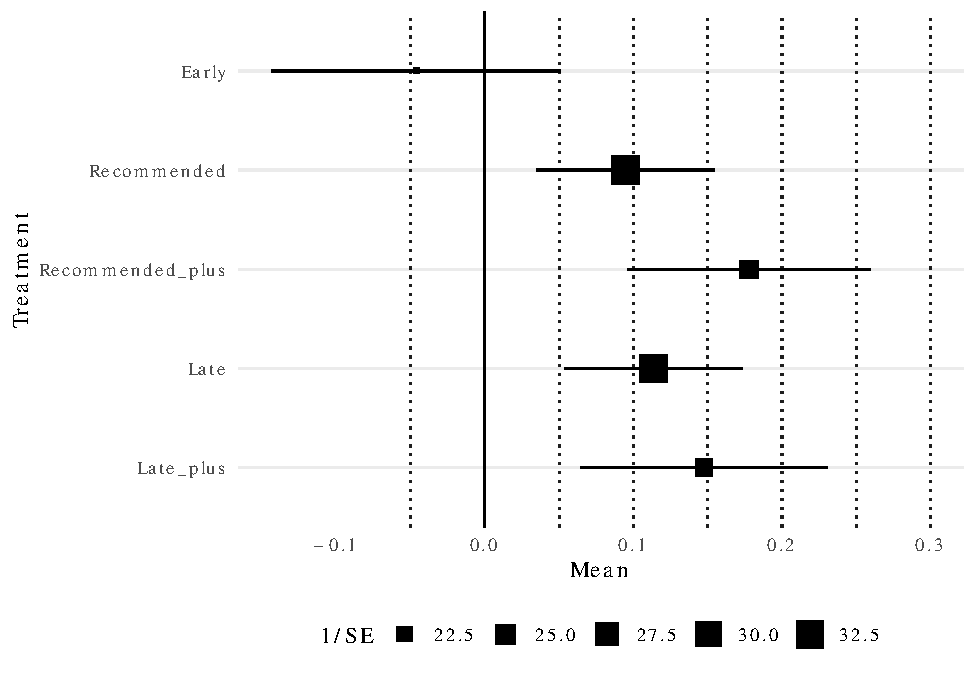
\includegraphics{paper_files/figure-latex/Figure1-1.pdf}

\hypertarget{results}{%
\section{Results}\label{results}}

\(control\), \(Early_{single}\), \(Recommended_{single}\),
\(Recommended_{plus}\), \(Late_{single}\), and \(Late_{plus}\).\\
Overall the meta-analysis indicated that, with the exception of the
\(Early_{single}\) treatment, all the the spray schedules were effective
at protecting mungbean yields relative to the no spray controls (Figure
@ref(fig:Figure1)). Treatments which incorporating multiple fungicide
applications, \(Recommended_{plus}\) and \(Late_{plus}\), produced the
highest mean yield protection estimates at 177.83 (SE = 41.69~kg~/~ha)
and 147.51~kg~/~ha (SE = 42.33~kg~/~ha) respectively (Table 3). Both
\(Recommended_{plus}\) and \(Late_{plus}\) were also significantly
higher than single applications \(Early_{single}\) (P = 0.0078 and P =
0.0025 respectively) and \(Late_{single}\)(P = 0.0476 and P = 0.0283
respectively). However, comparing \(Late_{plus}\) and \(Early_{single}\)
should done with caution given these treatments did not occur within the
same trial for any of the 15 trials included in the meta-analysis.
Within the single fungicide application treatments \texttt{Recommended}
provided the highest yield protection, and was estimated at saving an
average of 159.9 kg / ha (SE = 30.5 kg / ha) relative to the no spray
control (P \textless{} 0.0001). \texttt{Recommended} treatments were was
also significantly higher than \texttt{Early} treatments by 122.1 kg /
ha (SE = 42.1 kg / ha)(P = 0.004). Single \texttt{Late} applications
were effective at significantly mitigating the effect of powdery mildew
on yield by a mean of 122 kg / ha (SE = 39.2 kg / ha)(P = 0.0019).
However, this estimate was not significantly different to single
\texttt{Early} or \texttt{Recommended} treatments (P = 0.119; P = 0.278
respectively).

The \(Q_M\) omnibus test of moderators, shows the moderators
significantly influence the model (\(Q_M =\) 31.1217 \(,df =\) 5, P
\textless{} 0.0001) and we can reject the null hypothesis
(\(H_0 : \beta_1 = \beta_2 = \beta_3 =\beta_4 = 0\)) that there is no
difference between the moderators \citep{Viechtbauer2010}. The analysis
shows there is still a significant amount of residual heterogeneity
(\(Q_E =\) 37805.5158 \(,df=\) 149, P \textless{} 0.0001) not captured
by the spray management moderator indicating other possible moderators,
which might influence grain yield.

A log-ratio test, based on a chi-squared distribution, indicated that
retaining the \texttt{SpraySchedule} variable as a random interactive
term provided a significantly better model (P = 0.0179). An inspection
of log-likelihood profile plots showed the model, for each random
interactive term, provided a reasonable estimate of \(\tau^2\), with no
indication the variables were over-fit.

While the addition of disease pressure, as an interactive moderator term
to \texttt{SpraySchedule}, did explain slightly more residual
heterogeneity, shown by a lower \(Q_E = 409.91,\). The model including
disease pressure did not significantly improve the model (P = 0.4859)
and did not significantly explain differences in the
\texttt{SpraySchedule} term, and therefore disease pressure was not
included in the final model.

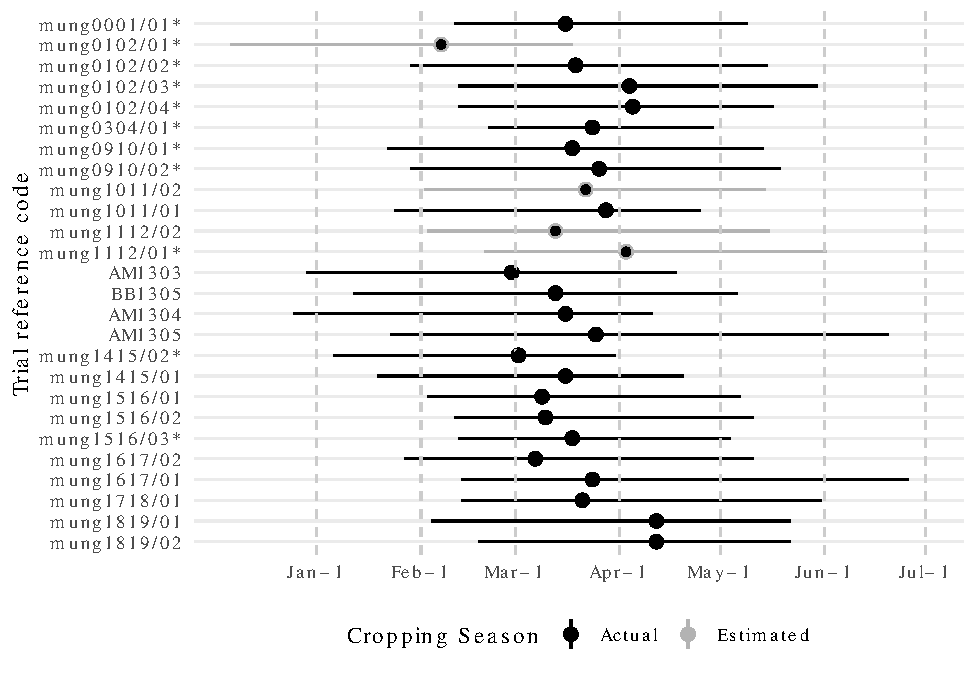
\includegraphics{paper_files/figure-latex/Figure2-1.pdf}

\begin{table}

\caption{\label{tab:table3_Contrasts}Estimated grain yield contrasts between each spray schedule.}
\centering
\begin{tabular}[t]{lrrrrl}
\toprule
Treatment contrasts & Estimate & Standard Error & Z-score & P-value &  \\
\midrule
Early - Recommended & 0.1221 & 0.0421 & 2.8990 & 0.0037 & **\\
Early - Recommended\_plus & 0.1587 & 0.0596 & 2.6617 & 0.0078 & **\\
Early - Late & 0.0843 & 0.0541 & 1.5595 & 0.1189 & \\
Early - Late\_plus & 0.1821 & 0.0603 & 3.0203 & 0.0025 & **\\
Recommended - Recommended\_plus & 0.0365 & 0.0371 & 0.9858 & 0.3242 & \\
\addlinespace
Recommended - Late & -0.0378 & 0.0349 & -1.0850 & 0.2779 & \\
Recommended - Late\_plus & 0.0600 & 0.0446 & 1.3445 & 0.1788 & \\
Recommended\_plus - Late & -0.0744 & 0.0375 & -1.9812 & 0.0476 & *\\
Recommended\_plus - Late\_plus & 0.0235 & 0.0453 & 0.5174 & 0.6049 & \\
Late - Late\_plus & 0.0978 & 0.0446 & 2.1932 & 0.0283 & *\\
\bottomrule
\multicolumn{6}{l}{\textit{Note: }}\\
\multicolumn{6}{l}{** - signficant at 0.005 level}\\
\multicolumn{6}{l}{* - signficant at 0.05 level}\\
\end{tabular}
\end{table}

\hypertarget{discussion}{%
\section{Discussion}\label{discussion}}

The current advice provided to growers for when to commence fungicide
applications for control of powdery mildew, is to spray at the first
sign of the disease then if necessary a follow-up spray two weeks later
\citep{SueThompson2016, Sparks2017}. This meta-analysis confirms that
advice, by showing that applying the first fungicide application, within
three days of first sign will significantly mitigate yield loss from
powdery mildew by between 34.89 to 154.78 kg / ha (\(Recommended\), P =
0.0019). In addition, spray schedules which commenced `late', up to 13
days after first sign of the disease were still effective at mitigating
yield loss by 53.5 to 173.64 kg / ha (\(Late\),P = 0.0002). Spray
schedules which included follow-up fungicide applications were on
average more effective at reducing yield loss due to powdery mildew by;
96.11 to 259.54 kg / ha in the \(RecommendedPlus\) treatments (P
\textless{} 0.0001) and 64.55 to 230.47 kg / ha in the \(LatePlus\)
treatments (P = 0.0005) (Figure @ref(fig:Figure2)) which again follows
the advice given by Thompson et al.~\citep{SueThompson2016}. This
meta-analysis adds certainty to the advice, which is currently given to
growers, especially around any uncertainty that Early sprays might be
effective at suppressing the disease. We show here Early fungicide
applications, which were made prior to any sign of the disease, were not
effective at mitigating yield loss.

This meta-analysis also provides a effective spray window for fungicide
applications, given that spray schedules, which commenced `late' were
still significantly effective at mitigating yield loss (\(Late\) P =
0.0002) 7 - 13 days after the first sign of disease. Growers typically
do not have the time to inspect their crop regularly for the first sign
of powdery mildew and therefore the disease may not be spotted within
the first couple of days of it establishing. Also, weather conditions
and logistical issues might prevent growers from getting machinery in
the paddock to treat the disease immediately after it is spotted. These
issues, and perhaps other on farm duties, might delay a timely
application, permitting the disease more time to establish. Knowing a
delay of up to two weeks may not lead to yield losses, can allow growers
to incorporate other integrated pest management options, such as
insecticide, with the fungicide spray saving on spray application costs.
However attention should be made to the label requirements when first
planning a spray schedule. Second applications, if they are needed,
should be applied at least 10 - 14 days after the first application and
not within 21 days of harvest \citep{APVMAcustodia}. If time permitted a
second spray after the first `late' application, on average the
meta-analysis shows this would be optimal, as the \(LatePlus\) treatment
significantly limited yield loss by 97.8 kg / ha, when compared to the
\(Late\), single spray treatment P = 0.0283.

It is important to note, the studies included in this meta-analysis may
not reflect a `normal' mungbean season. All the included experiments
were intentionally sown late in the season, from January through to as
late as early March, to ensure powdery mildew infection (Figure
@ref(fig:Figure2)). While certain circumstances may force growers to sow
mungbeans late, many may decide to fallow their fields instead of
risking a powdery mildew epidemics and an early frost damaging the crop
and yields. Regardless, according to the Australian Mungbean Association
sowing guide \citep{AMAplanting}, mungbeans should not be sown later
than January in the Darling Downs, the region where the majority of
trials were undertaken. If the planting guide is adhered to the mungbean
would be at a lower risk of powdery mildew, reducing the requirement for
fungicide applications. An example of this is if we inspect the six
trials in which powdery mildew manifested 60 days or greater after
planting (Trial references: AM1304, mung1819/01, mung1011/01, AM1303,
AM1305 and BB1305). Of these trials, four directly compared single
\(Recommended\) fungicide applications and \(RecommendedPlus\) (AM1303,
AM1305, BB1305 and mung1819/01), two of which (AM1305 and mung1819/01)
produced at least one treatment \(RecommendedPlus\) treatment with a
higher grain yield the \(Recommended\) treatments. However, neither
AM1305 or mung1819/01 neither contained \(Recommended\) or
\(RecommendedPlus\) treatments with higher mean yields than the no-spray
control. This indicating there is likely no benefit to applying two
fungicide applications when the disease manifests later than 60 days
into the growing season. Further the trials undertaken in 2013, such as
Premer (AM1303), Goolhi (AM1305) Marys Mount (AM1304) and Millmerran
(BB1305) reported a significant difference in powdery mildew severity
between the fungicide treatments, however neither trial showed a
significant difference in grain yield between treatments
\citep[\citet{premer2013}, \citet{Marysmount2013},
\citet{goolhi2013}]{Millmerran2013}. Therefore, discretion is still
required for if fungicide applications are necessary given the crop
growth stage and forecast weather conditions. The PowderyMildewMBM
considers crop growth stage and weather, to assist decision making
whether to spray or not to spray \citep{Diggle}.

PowderyMildewMBM also provides a cost-benefit analysis to growers for
fungicide spray schedule scenarios. The user inputs weather, crop, and
economic inputs into the DSS and the application returns the probability
that one or two fungicide sprays would protect yields sufficiently to
increase the net profit. The scope of the meta-analysis is limited to
the timing of fungicide application and therefore we can't validate all
the variables available in PowderyMildewMBM. However our results
validate the decision of the app developers not to recommend
prophylactic fungicide applications. If the powdery mildew is not
observed in the crop the app advises the user to keep monitoring for
disease.\\

Scouting the crop for powdery mildew might not be necessary during the
warmer months of the season. Data from the trials included in this
experiment show regardless of crop sowing date, powdery mildew
establishes on average in the month of March, which marks the beginning
of autumn (Figure @ref(fig:Figure2)). Considering the results of the
meta-analysis, weekly inspections would be ideal to ensure timely
fungicide applications if necessary. Scouting at intervals greater than
12 - 13 days, might risk crop losses if a spray schedule does not
commence within aforementioned the spray window. More work is needed to
understand when `late' fungicide applications are too late.

We estimate the costs of applying tebuconazole fungicide at \$4.18 AUD /
ha, if fungicide is purchased at \$15 / L \citep{Simfendorfer2011} and
applications cost are
\(2 per hectare [@QueenslandGovernment2019]. The meta-analysis estimates average yield savings of between kg / ha (\)Recommended\() and kg / ha (\)RecommendedPlus\$).
These average yield savings would save \$ AUD / ha for a single
application at first sign and AUD / ha if a follow-up application is
made. Lucrative returns such as these may tempt growers into applying
fungicide to control diseases such as powdery mildew when they are
unnecessary. Excessive use of fungicides are highly likely to lead
ongoing problems such as fungicide resistance. \emph{Podosphaera
xanthii} is categorised by the Australian Fungicide resistance Action
Committee (FRAC) as a `High risk' candidate to evolve fungicide
resistance \citep{FRACrisk2019}. Evolution of fungicide resistance can
occur quickly, especially when spray schedules are not designed with
potential fungicide resistance in mind. Powdery mildew is one such group
of fungal pathogens with an extensive track record of rapidly developing
fungicide resistance. In cucurbits, \emph{P. xanthii} evolved resistance
to benzimidazole within three years of its registration
\citep{Peterson1973} and has evolved resistance to numerous fungicide
classes, such as benzimidazoles, demethylation inhibitors,
organophosphates, hydroxypyrimidines, quinone inhibitors and
quinoxalines since \citep{Mcgrath2001}. In cereal crops \emph{Blumeria
graminis} showed reduced sensitivity to strobilurins in 1998, two years
after the fungicides began being used in Europe \citep{Chin2001}.

According to the Fungicide Resistance Action Committee (FRAC) it is
important to alternate or mix fungicides with different modes of action
to avoid fungicide resistance. At the time of writing, in Australia one
fungicide is registered with the to treat powdery mildew in mungbean,
Veritas/Custodia (200 g/L tebuconazole with 120 g/L azoxystrobin). This
fungicide provides dual action: tebeconazole disrupts C-14 demethylase,
required in sterol biosynthesis for cell membranes; and azoxystrobin, a
Quinone outside inhibitor. Quinone is required in cell metabolism and
active in the mitochondrial complex III. However FRAC recommends that
applications of QoIs or strobilurins, singularly or as a mixture, should
not be applied consecutively and alternated with a fungicide from a
different group \citep{Brent2007}. For mungbean, past experiments have
shown some success with sulphur applications to control powdery mildew.
Sulphur is a non-systemic protectant and thus provides an excellent
option for rotation to limit the emergence of fungicide resistance.

To extend the time that a fungicide remains effective against the target
pathogen, strategic use of the fungicide must be considered. Excessive
fungicide sprays by a single active increase the selection pressure on
the pathogen to evolve resistance \citep{Brent2007}. If any strains of
the pathogen with resistance to the fungicide are present in a
population regular use of the fungicide will increase it's proportion in
the population. Therefore, managing the disease with fungicides for the
highest economic return is likely not to require eradication of the
causal pathogen. Integrated pest management practices focus on using
only the required number of chemical control to protect the economic
return. These strategies permit the presence of yield limiting diseases
and pests if intervening would cost more than the economic return of
protection.

Advising use of fungicide for disease control to protect yields should
also consider the harm it may do to symbiotic relationships with
microbiota. While some nitrogen fixing symbiont show a level of
tolerance to fungicides, all are detrimentally affected by increasing
concentrations of fungicide leading to lower nodulation and biomass
accumulation \citep[\citet{Shahid2019}]{Ahemad2011}. Therefore if a
grower is relying on inoculating with rhizobia to help meet the crops
nitrogen requirements, untimely and excessive applications of a systemic
fungicide for powdery mildew control may actually reduce yield.

\hypertarget{future-work}{%
\subsection{Future work}\label{future-work}}

This meta-analysis provides a ballast for the direction of future
powdery mildew research in mungbean. However it does not provide enough
certainty to when late fungicide applications would be too late to
protect yield losses due to the disease. Future experiments should take
note of physiological maturity of the crop throughout the season so
`crop age' might be considered as a covariate in future analyses. In
cases where mungbean physiological maturity may not have been recorded
the APSIM mungbean module \citep{RobertsonAPSIMlegume2002}.

Early detection of powdery mildew is vital for an effective fungicidal
control response. Data from the collection of 26 studies in the Northern
Grain region, indicate powdery mildew is likely to manifest on crops in
the first month of autumn. This data together with additional
observations may permit models to predict the likely onset of the
disease given weather parameters, providing an early warning system for
growers to scout their crop for signs of powdery mildew. However an
improved understanding of the pathogen biology is also needed to ensure
models are as accurate as they can be. The population genetics,
epidemiology and alternate hosts are all poorly understood in this
host-pathogen relationship. The recent discovery of a second powdery
mildew species, which infects mungbean highlights the paucity of
knowledge on this disease.

\hypertarget{conclusion}{%
\section{Conclusion}\label{conclusion}}

\hypertarget{supplemental-material}{%
\section{Supplemental Material}\label{supplemental-material}}

Supplementary material can be found in the following research
compendium.

\hypertarget{data-availability}{%
\section{Data Availability}\label{data-availability}}

All data and code used in the preparation of this manuscript can be
found in the associated research compendium.

\hypertarget{conflict-of-interest-statement}{%
\section{Conflict of Interest
Statement}\label{conflict-of-interest-statement}}

The authors of this paper have no conflicting interest in the research
presented in this manuscript

\hypertarget{acknowledgments}{%
\section{Acknowledgments}\label{acknowledgments}}

The authors wish to acknowledge the work done by Professor Malcolm Riley
and Dr Sue Thompson whom undertook many of the trials incorporated in
this analysis from 2004 - 2015. The Queensland Department of
Agriculture, Fisheries and Forestry (DAF). The National Growers
association and Lawrie Price for contributing data. The Grains Research
and Development Corporation who funded this research.

% %%%%%%%%%%%%%%%%%%%%%%%%%%%%%%%%%%%%%%%%%%
% %% optional
% \supplementary{The following are available online at www.mdpi.com/link, Figure S1: title, Table S1: title, Video S1: title.}
%
% % Only for the journal Methods and Protocols:
% % If you wish to submit a video article, please do so with any other supplementary material.
% % \supplementary{The following are available at www.mdpi.com/link: Figure S1: title, Table S1: title, Video S1: title. A supporting video article is available at doi: link.}

\vspace{6pt}

%%%%%%%%%%%%%%%%%%%%%%%%%%%%%%%%%%%%%%%%%%
\acknowledgments{All sources of funding of the study should be
disclosed. Please clearly indicate grants that you have received in
support of your research work. Clearly state if you received funds for
covering the costs to publish in open access.}

%%%%%%%%%%%%%%%%%%%%%%%%%%%%%%%%%%%%%%%%%%
\authorcontributions{For research articles with several authors, a short
paragraph specifying their individual contributions must be provided.
The following statements should be used ``X.X. and Y.Y. conceive and
designed the experiments; X.X. performed the experiments; X.X. and Y.Y.
analyzed the data; W.W. contributed reagents/materials/analysis tools;
Y.Y. wrote the paper.'\,' Authorship must be limited to those who have
contributed substantially to the work reported.}

%%%%%%%%%%%%%%%%%%%%%%%%%%%%%%%%%%%%%%%%%%
\conflictsofinterest{Declare conflicts of interest or state `The authors
declare no conflict of interest.' Authors must identify and declare any
personal circumstances or interest that may be perceived as
inappropriately influencing the representation or interpretation of
reported research results. Any role of the funding sponsors in the
design of the study; in the collection, analyses or interpretation of
data in the writing of the manuscript, or in the decision to publish the
results must be declared in this section. If there is no role, please
state `The founding sponsors had no role in the design of the study; in
the collection, analyses, or interpretation of data; in the writing of
the manuscript, an in the decision to publish the results'.}

%%%%%%%%%%%%%%%%%%%%%%%%%%%%%%%%%%%%%%%%%%
\funding{Please add:
\texttt{This\ research\ received\ no\ external\ funding\textquotesingle{}\textquotesingle{}\ or}This
research was funded by NAME OF FUNDER grant number XXX.'\,' and ``The
APC was funded by XXX'\,'. Check carefully that the details given are
accurate and use the standard spelling of funding agency names at
\url{https://search.crossref.org/funding}, any errors may affect your
future funding.}

%%%%%%%%%%%%%%%%%%%%%%%%%%%%%%%%%%%%%%%%%%
%% optional
\abbreviations{The following abbreviations are used in this manuscript:\\

\noindent
\begin{tabular}{@{}ll}
MDPI & Multidisciplinary Digital Publishing Institute \\
DOAJ & Directory of open access journals \\
TLA & Three letter acronym \\
LD & linear dichroism \\
\end{tabular}}


%%%%%%%%%%%%%%%%%%%%%%%%%%%%%%%%%%%%%%%%%%
% Citations and References in Supplementary files are permitted provided that they also appear in the reference list here.

%=====================================
% References, variant A: internal bibliography
%=====================================
%\reftitle{References}
%\begin{thebibliography}{999}
% Reference 1
%\bibitem[Author1(year)]{ref-journal}
%Author1, T. The title of the cited article. {\em Journal Abbreviation} {\bf 2008}, {\em 10}, 142--149.
% Reference 2
%\bibitem[Author2(year)]{ref-book}
%Author2, L. The title of the cited contribution. In {\em The Book Title}; Editor1, F., Editor2, A., Eds.; Publishing House: City, Country, 2007; pp. 32--58.
%\end{thebibliography}

% The following MDPI journals use author-date citation: Arts, Econometrics, Economies, Genealogy, Humanities, IJFS, JRFM, Laws, Religions, Risks, Social Sciences. For those journals, please follow the formatting guidelines on http://www.mdpi.com/authors/references
% To cite two works by the same author: \citeauthor{ref-journal-1a} (\citeyear{ref-journal-1a}, \citeyear{ref-journal-1b}). This produces: Whittaker (1967, 1975)
% To cite two works by the same author with specific pages: \citeauthor{ref-journal-3a} (\citeyear{ref-journal-3a}, p. 328; \citeyear{ref-journal-3b}, p.475). This produces: Wong (1999, p. 328; 2000, p. 475)

%=====================================
% References, variant B: external bibliography
%=====================================
\reftitle{References}
\externalbibliography{yes}
\bibliography{../Mungbean.bib}

%%%%%%%%%%%%%%%%%%%%%%%%%%%%%%%%%%%%%%%%%%
%% optional
\sampleavailability{Samples of the compounds \ldots\ldots{} are
available from the authors.}

%% for journal Sci
%\reviewreports{\\
%Reviewer 1 comments and authors’ response\\
%Reviewer 2 comments and authors’ response\\
%Reviewer 3 comments and authors’ response
%}

%%%%%%%%%%%%%%%%%%%%%%%%%%%%%%%%%%%%%%%%%%
\end{document}
